\newpage
\subsection{Ghi log bảo mật}

\subsubsection*{Mục tiêu}
Chức năng ghi log bảo mật nhằm đảm bảo toàn bộ hành động của người dùng và các sự kiện nội bộ trong hệ thống đều được theo dõi, ghi nhận và lưu trữ dưới dạng thống nhất. Việc này phục vụ:
\begin{itemize}
    \item Truy vết các hành động quan trọng: đăng nhập, ký số, xác minh,...
    \item Giám sát lỗi bảo mật và cảnh báo bất thường.
    \item Làm bằng chứng trong điều tra sự cố hoặc kiểm toán.
\end{itemize}

\subsubsection*{Giao diện}
Giao diện tại trang \texttt{/admin\_dashboard} cung cấp:
\begin{itemize}
    \item Bảng hiển thị đầy đủ log: thời gian, mức độ (INFO, WARNING, ERROR), email người dùng, hành động, trạng thái và chi tiết.
    \item Tính năng tìm kiếm realtime và nút \texttt{Reload} để làm mới dữ liệu.
    \item Dữ liệu được render động thông qua fetch \texttt{X-Requested-With = XMLHttpRequest}.
\end{itemize}

\begin{figure}[H]
    \centering
    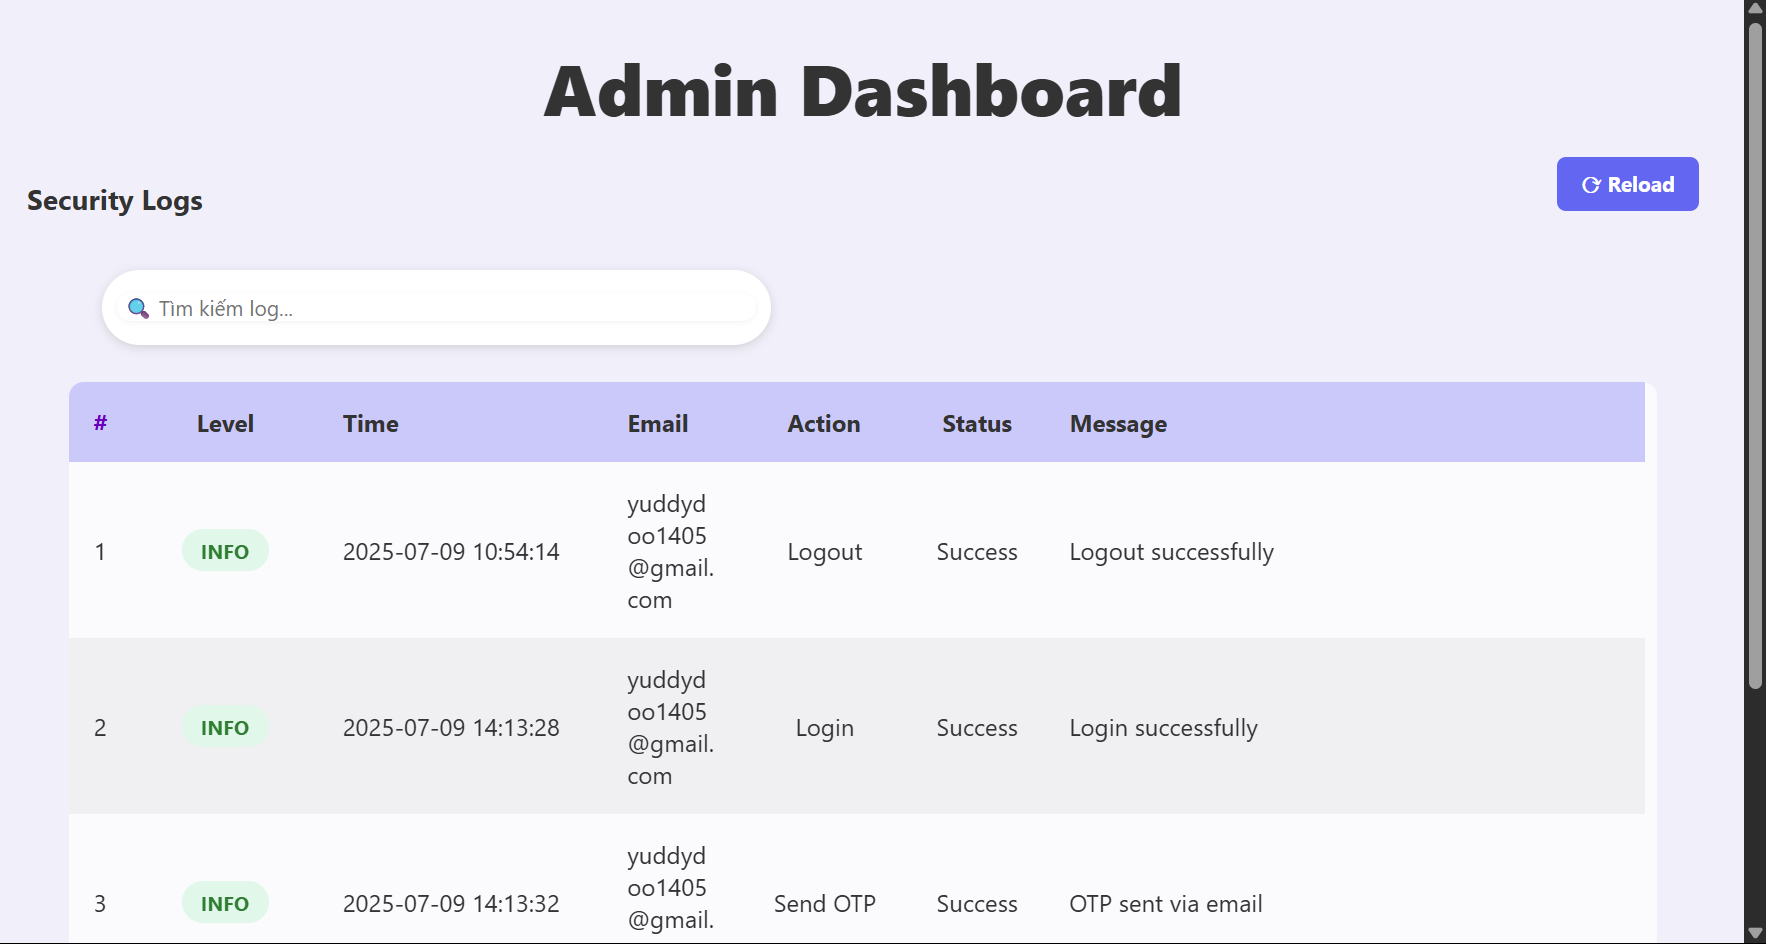
\includegraphics[width=0.85\textwidth]{img/11_logger/11_logger_table.png}
    \caption{Bảng log của admin}
\end{figure}

\subsubsection*{Quy trình thực hiện}
\begin{description}
    \item[\textbf{1. Người dùng thực hiện hành động}]
    Mỗi khi người dùng thao tác (ví dụ: đăng nhập, ký file, xác minh), hàm \texttt{log\_user\_action()} được gọi để ghi log với thông tin đầy đủ: email, hành động, trạng thái, chi tiết và mức độ severity.

    \begin{figure}[H]
        \centering
        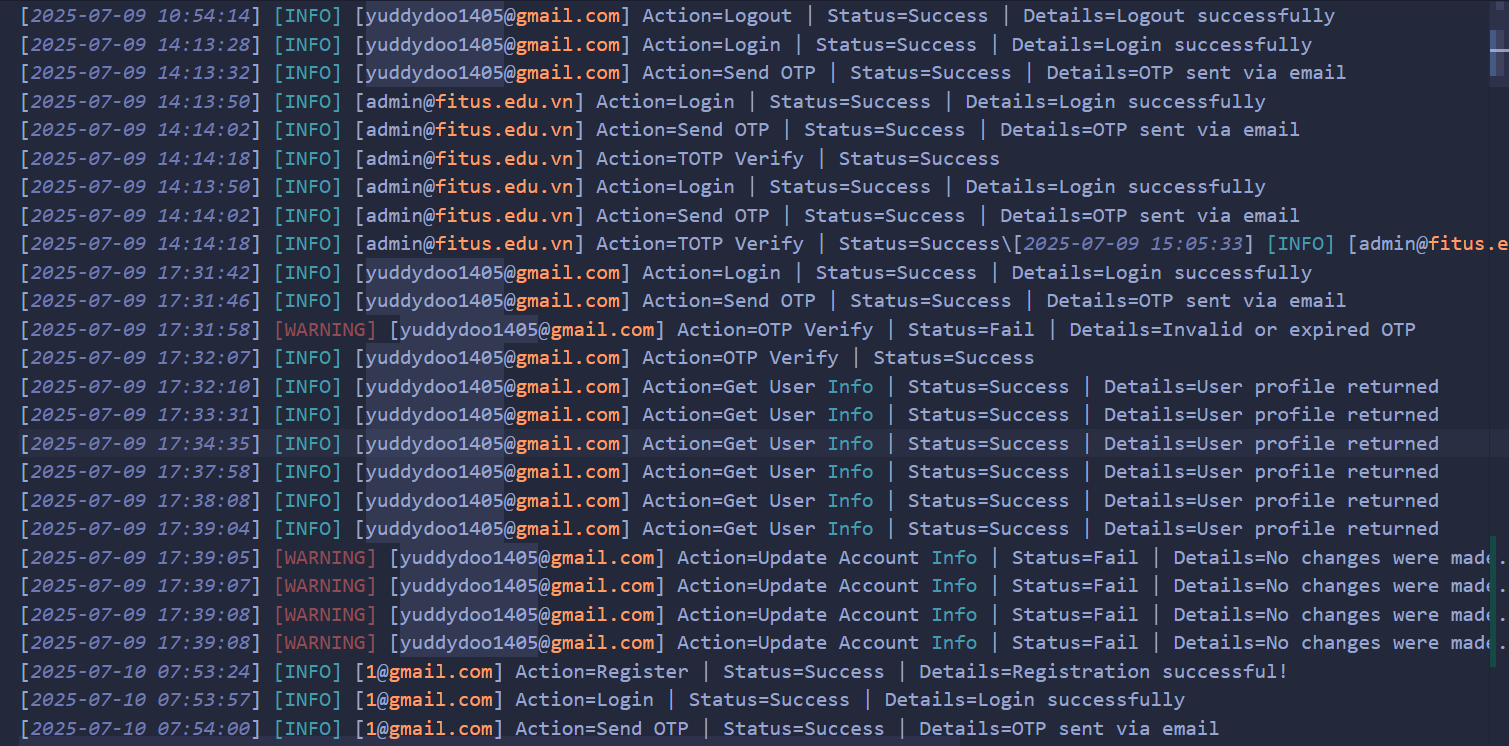
\includegraphics[width=0.85\textwidth]{img/11_logger/11_logger_file.png}
        \caption{Log cho người dùng - Routes}
    \end{figure}

    \item[\textbf{2. Hệ thống nội bộ phát sinh sự kiện}]
    Các module nội bộ (như mã hóa, xác minh chữ ký) có thể gọi \texttt{log\_internal\_event()} để ghi lại log kỹ thuật chi tiết.
    \begin{figure}[H]
        \centering
        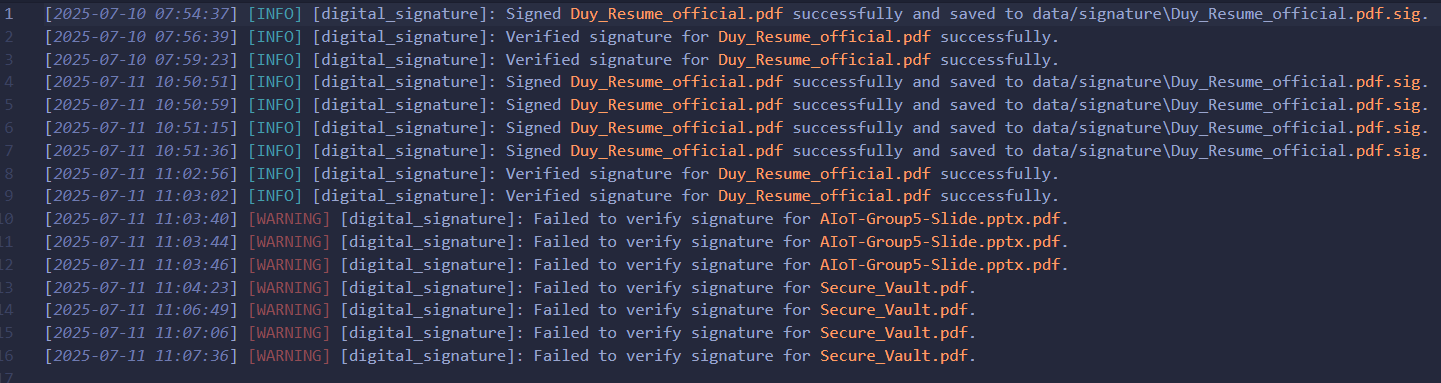
\includegraphics[width=0.85\textwidth]{img/11_logger/11_logger_debug.png}
        \caption{Log cho debug - Modules}
    \end{figure}

    \item[\textbf{3. Lưu vào file log}]
    Log người dùng và log nội bộ để debug sẽ được lưu vào các file riêng
    \begin{itemize}
        \item Log người dùng được ghi vào \texttt{log/security.log}
        \item Log module nội bộ được ghi vào \texttt{log/debug\_log.log}
    \end{itemize}

    \item[\textbf{4. Giao diện đọc log}]
    Khi người dùng truy cập trang \texttt{/admin\_dashboard}, Flask route đọc và phân tích nội dung từ file log, chuyển thành danh sách JSON và hiển thị trên giao diện.
\end{description}

\subsubsection*{Chi tiết kỹ thuật và thư viện bảo mật}
\begin{description}

    \item[\textbf{1. Hàm log người dùng}]
    \texttt{log\_user\_action(email, action, status, details, level)} ghi log theo format thống nhất:
    \begin{itemize}
        \item Ví dụ log: \texttt{[2025-07-09 10:15:23] [INFO] [user@example.com] Action=Sign File | Status=Success | Details=file=report.pdf}
        \item Sử dụng thư viện chuẩn \texttt{logging}, ghi vào \texttt{log/security.log}
    \end{itemize}

    \item[\textbf{2. Log nội bộ hệ thống}]
    \texttt{log\_internal\_event(module, message, level)} dùng cho debug các module như crypto, xác minh,...
    \begin{itemize}
        \item Ví dụ: \texttt{[crypto]: Signature verified successfully.}
        \item Ghi vào \texttt{log/debug\_log.log} với format chi tiết hơn để phục vụ debug.
    \end{itemize}

    \item[\textbf{3. Route hiển thị log}]
    Route \texttt{/log\_security} thực hiện:
    \begin{itemize}
        \item Đọc file \texttt{log/security.log}, tách thành các trường: \texttt{timestamp, level, user, action, status, details}
        \item Trả về \texttt{JSON} nếu là AJAX, hoặc render giao diện nếu là truy cập thường
    \end{itemize}

    \item[\textbf{4. Mức độ log hỗ trợ}]
    \begin{itemize}
        \item \texttt{INFO} – hành động thành công hoặc hợp lệ
        \item \texttt{WARNING} – thao tác sai, lỗi thường gặp
        \item \texttt{ERROR} – lỗi hệ thống hoặc dữ liệu bất thường
        \item \texttt{DEBUG} – dành cho log kỹ thuật nội bộ (chỉ module log mới dùng)
    \end{itemize}

    \item[\textbf{5. Định dạng và chuẩn hóa log}]
    Mọi log đều tuân thủ format:
    \begin{quote}
        \texttt{[timestamp] [LEVEL] [email] Action=... | Status=... | Details=...}
    \end{quote}
    Điều này giúp dễ dàng phân tích bằng tool, lọc log, và hỗ trợ audit.

\end{description}
